%%%%%%%%%%%%%%%%%%%%%%%%%%%%%%%%%%%%%%%%%%%%%%%%%%%%%%%%%%%%%%%%%%%%%%%%%%%
% Copyright (c) 2010 committers of YAKINDU and others.
% All rights reserved. This program and the accompanying materials
% are made available under the terms of the Eclipse Public License v1.0
% which accompanies this distribution, and is available at
% http://www.eclipse.org/legal/epl-v10.html
%
% Contributors:
%     committers of YAKINDU - initial API and implementation
%%%%%%%%%%%%%%%%%%%%%%%%%%%%%%%%%%%%%%%%%%%%%%%%%%%%%%%%%%%%%%%%%%%%%%%%%%%
\section{Integrating Generated Java Code}

A demonstration example that reflects the integration of the Java code,
generated for the \emph{TrafficLight} example with manually written code is
deployed with the YAKINDU Statechart tools and may be created using the
example wizard as outlined by Figures \ref{fig:screenshot17} and
\ref{fig:screenshot18}.

\begin{figure}[h!]
\center
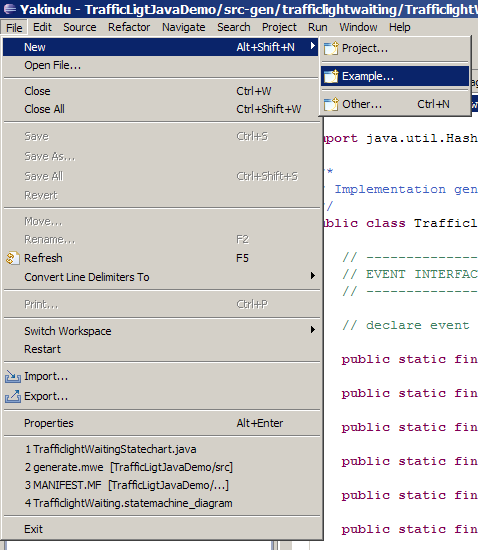
\includegraphics[width=0.45\textwidth]{./Pictures/Screenshot17}
\caption{\label{fig:screenshot17} Opening the Example Wizard}
\end{figure}


\begin{figure}[h!]
\center
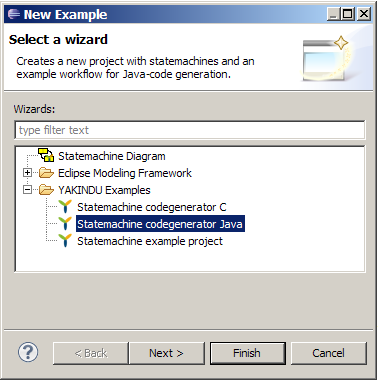
\includegraphics[width=0.5\textwidth]{./Pictures/Screenshot18}
\caption{\label{fig:screenshot18} Creating a new Java Code Generator Example Project}
\end{figure}

\clearpage
As depicted by Figure \ref{fig:screenshot19} it contains some manually written
code (within the \texttt{src} folder) that realizes a Draw2d visualization of
a traffic light, being adapted (within the \texttt{CrossingDemo} main class)
to the generated source code of the \emph{TrafficLight} example (contained in
the \texttt{src-gen} folder of the example project).

\begin{figure}[h!]
\center
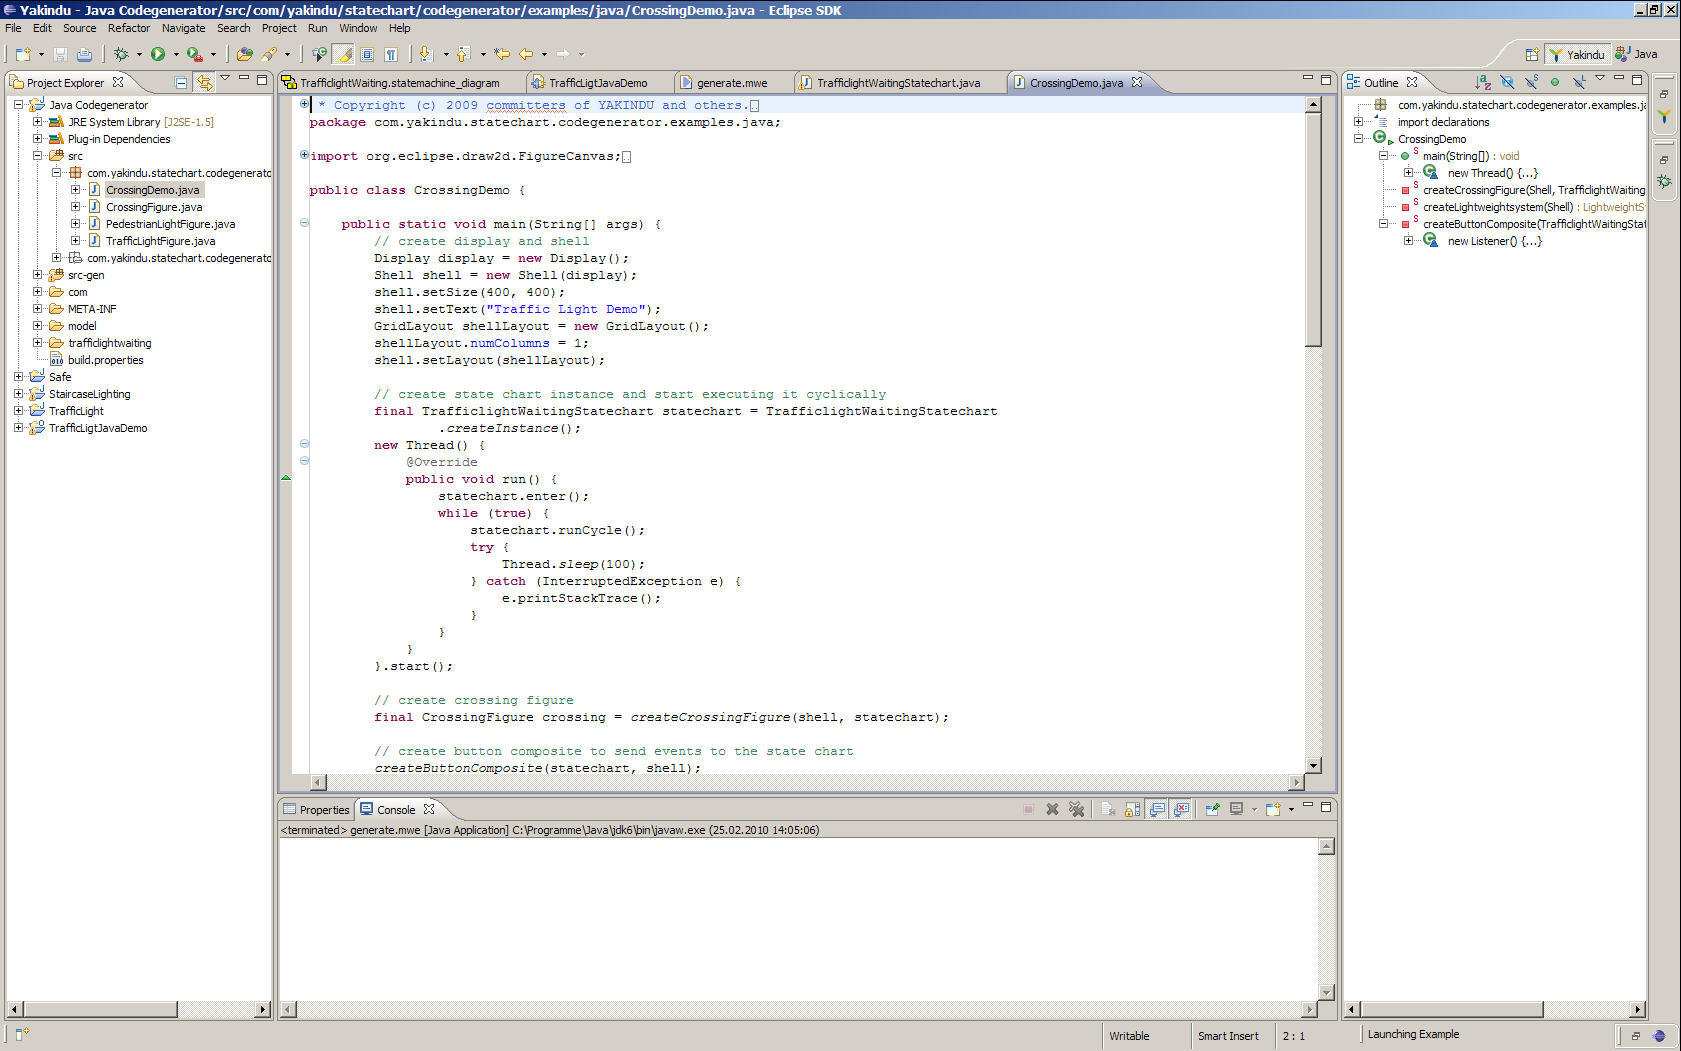
\includegraphics[width=\textwidth]{./Pictures/Screenshot19}
\caption{\label{fig:screenshot19} Traffic Light Java Demo Project Contents}
\end{figure}

\clearpage
As outlined in Figures \ref{fig:screenshot20} and \ref{fig:screenshot21}, the
\texttt{CrossingDemo} main class within the example project may be executed as
a Java application. It shows a visualization of the \emph{TrafficLight} state
chart variable values (by means of colors of the traffic and pedestrian lights
contained) and offers a button group, which prolongs respectively named events
to the \emph{TrafficLight} state chart.

\begin{figure}[h!]
\center
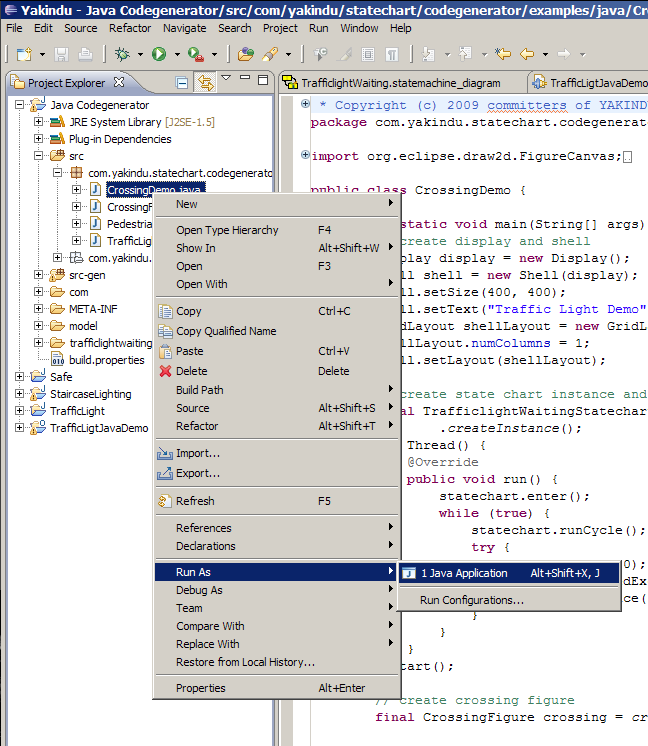
\includegraphics[width=0.45\textwidth]{./Pictures/Screenshot20}
\caption{\label{fig:screenshot20} Running CrossingDemo as Java Application}
\end{figure}

\begin{figure}[h!]
\center
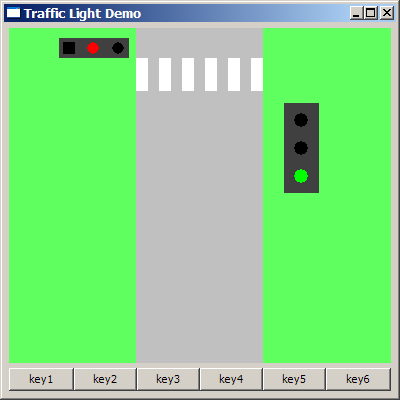
\includegraphics[width=0.5\textwidth]{./Pictures/Screenshot21}
\caption{\label{fig:screenshot21} CrossingDemo Application}
\end{figure}